\chapter{Preventivo}

\section{Verso la RTB}

\subsection{Primo periodo}

In questa fase i ruoli da ricoprire per portare a termine gli obiettivi
pianificati sono:
\begin{itemize}
    \item \textit{Responsabile};
    \item \textit{Amministratore};
    \item \textit{Verificatore}.
\end{itemize}

\subsubsection{Preventivo orario}

\begin{table}[H]
    \centering
    \begin{tabular}{|l|c|c|c|c|c|c|c|}
    \hline
    \textbf{Membro} & \multicolumn{1}{l|}{\textbf{RE}} & \multicolumn{1}{l|}{\textbf{AM}} & \multicolumn{1}{l|}{\textbf{AN}} & \multicolumn{1}{l|}{\textbf{PT}} & \multicolumn{1}{l|}{\textbf{PR}} & \multicolumn{1}{l|}{\textbf{VE}} & \multicolumn{1}{l|}{\textbf{Totale ore persona}} \\ \hline
    \textit{Marco Mazzucato}  & 2 & 3  & - & - & - & 1 & 6  \\ \hline
    \textit{Marco Mamprin}    & - & 3  & - & - & - & 1 & 4  \\ \hline
    \textit{Marko Vukovic}    & 2 & 3  & - & - & - & 1 & 6  \\ \hline
    \textit{Mattia Zanellato} & - & 3  & - & - & - & 1 & 4  \\ \hline
    \textit{Emanuele Pase}    & - & 3  & - & - & - & 1 & 4  \\ \hline
    \textit{Riccardo Contin}  & - & 3  & - & - & - & 1 & 4  \\ \hline
    \textit{Lorenzo Onelia}   & - & 3  & - & - & - & 1 & 4  \\ \hline
    \textbf{Totale ore ruolo} & 4 & 21 & - & - & - & 7 & 32 \\ \hline
    \end{tabular}
    \caption{Distribuzione delle ore per la prima milestone}
\end{table}

\begin{figure}[H]
    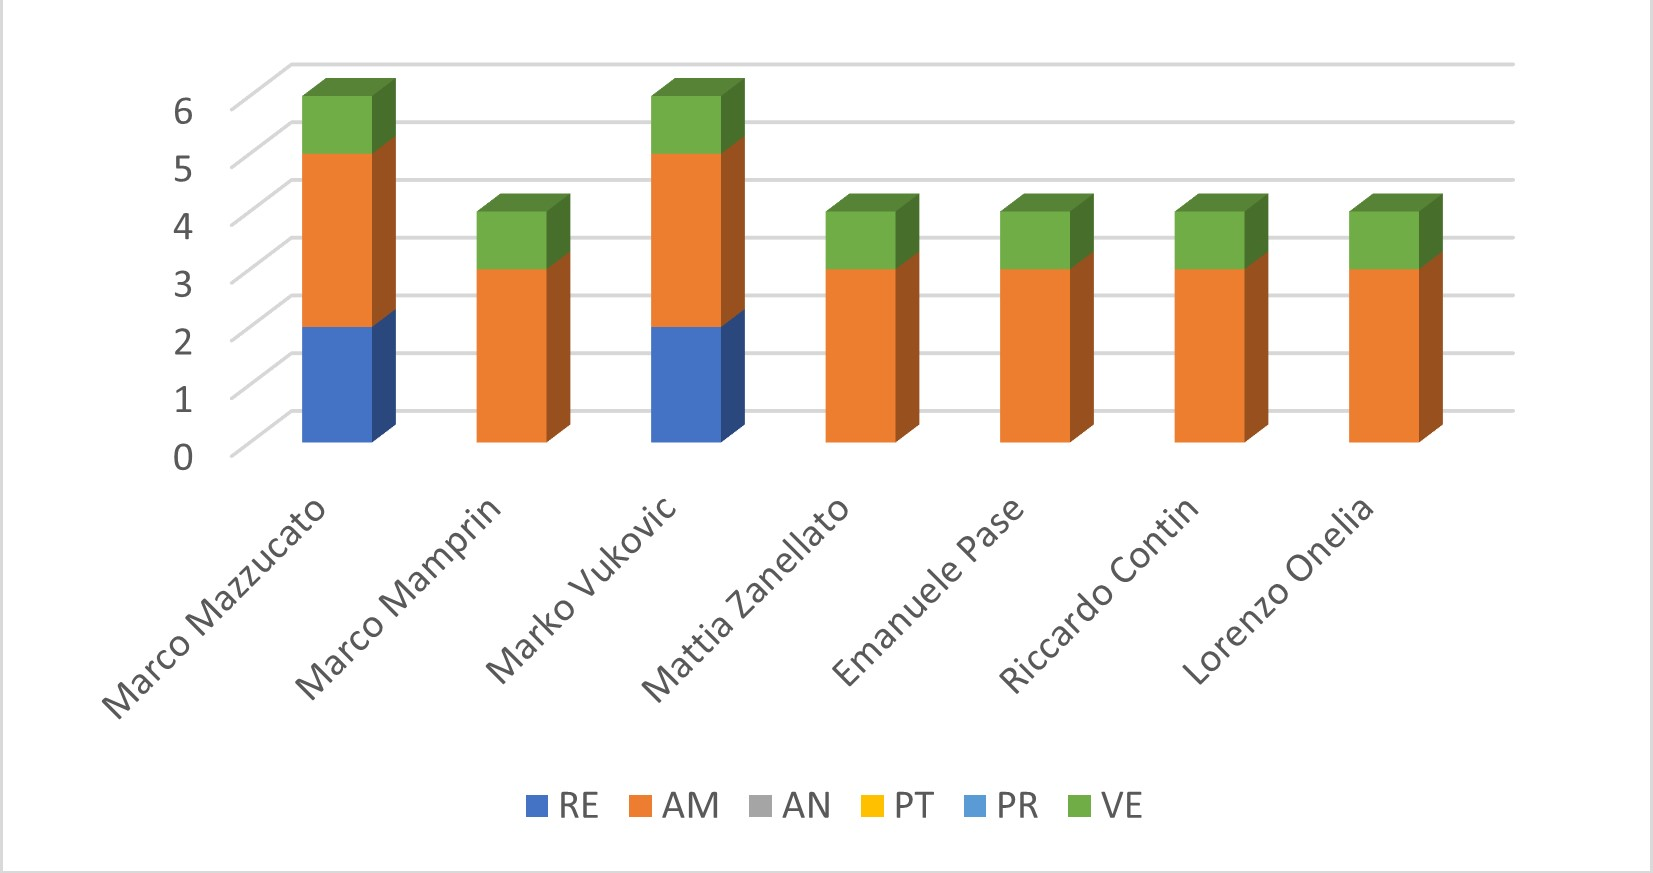
\includegraphics[width=1.0\textwidth]{Istogramma1.jpg}
    \caption{Istogramma della distribuzione delle ore}
\end{figure}

\begin{figure}[H]
    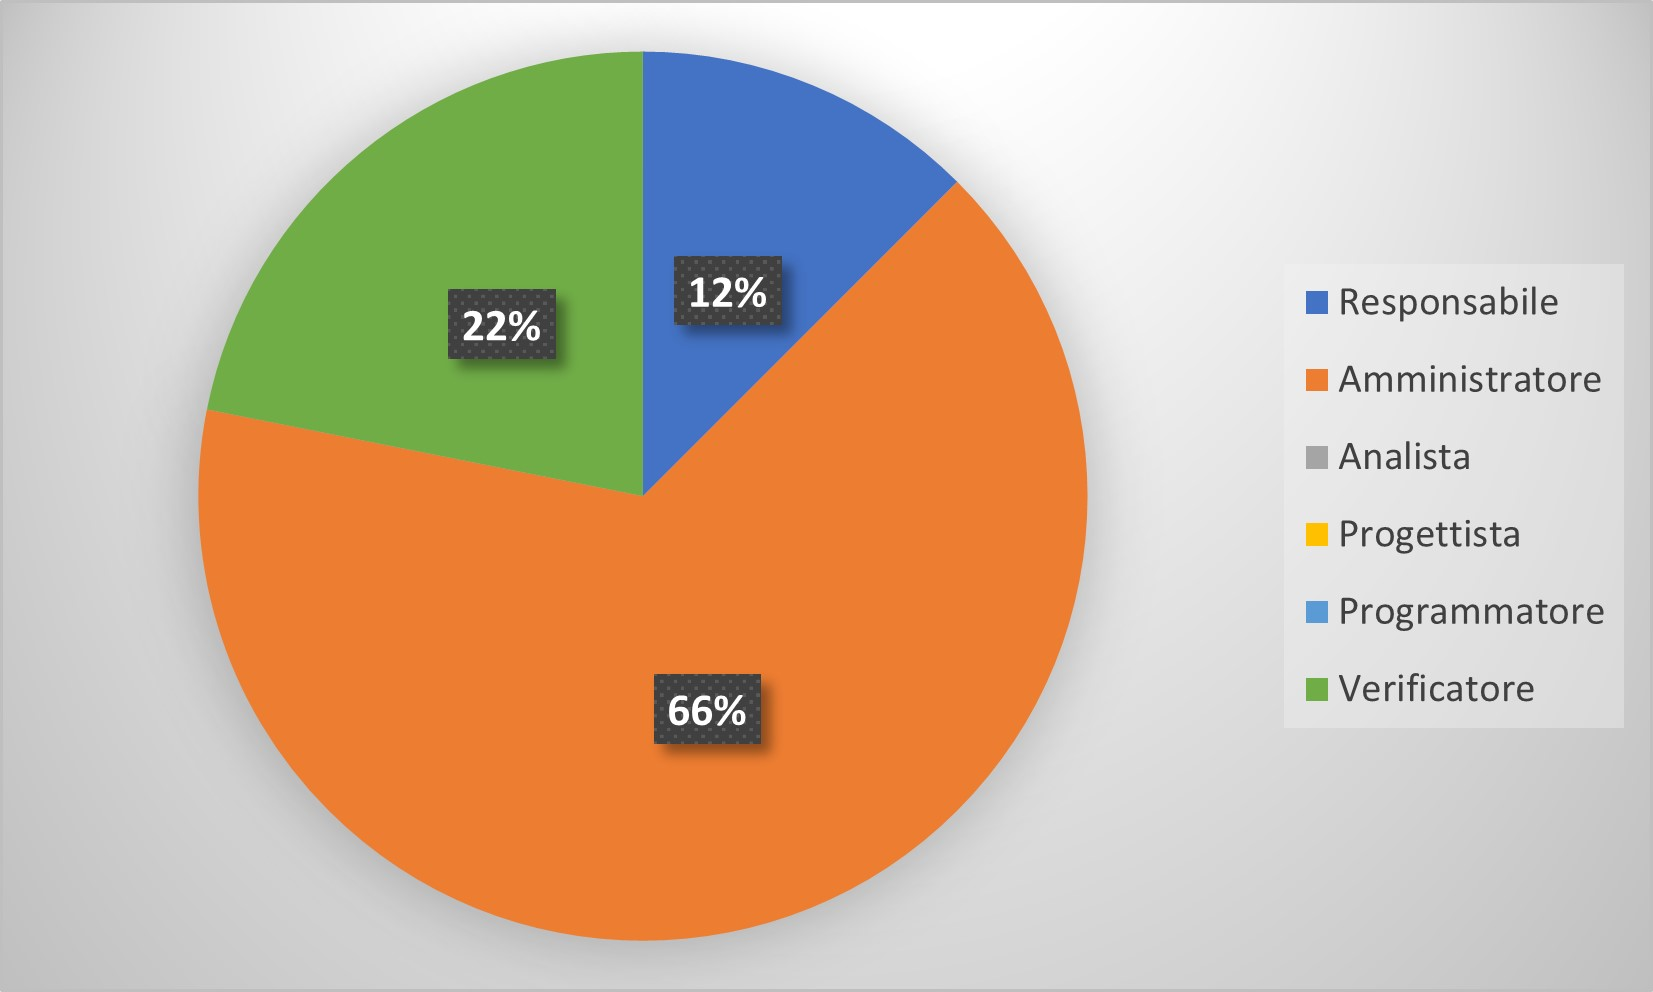
\includegraphics[width=1.0\textwidth]{Torta1.1.jpg}
    \caption{Grafico a torta della distribuzione delle ore}
\end{figure}

\newpage
\subsubsection{Preventivo economico}

\begin{table}[H]
    \centering
    \begin{tabular}{|l|c|c|}
    \hline
    \textbf{Ruolo} & \multicolumn{1}{l|}{\textbf{Ore}} & \multicolumn{1}{l|}{\textbf{Costo (€)}} \\ \hline
    \textit{Responsabile} & 4 & 120 \\ \hline
    \textit{Amministratore} & 21 & 420 \\ \hline
    \textit{Analista} & - & - \\ \hline
    \textit{Progettista} & - & - \\ \hline
    \textit{Programmatore} & - & - \\ \hline
    \textit{Verificatore} & 7 & 105 \\ \hline
    \textbf{Totale} & 32 & 645 \\ \hline
    \end{tabular}
    \caption{Prospetto dei costi per la prima milestone}
\end{table}

\begin{figure}[H]
    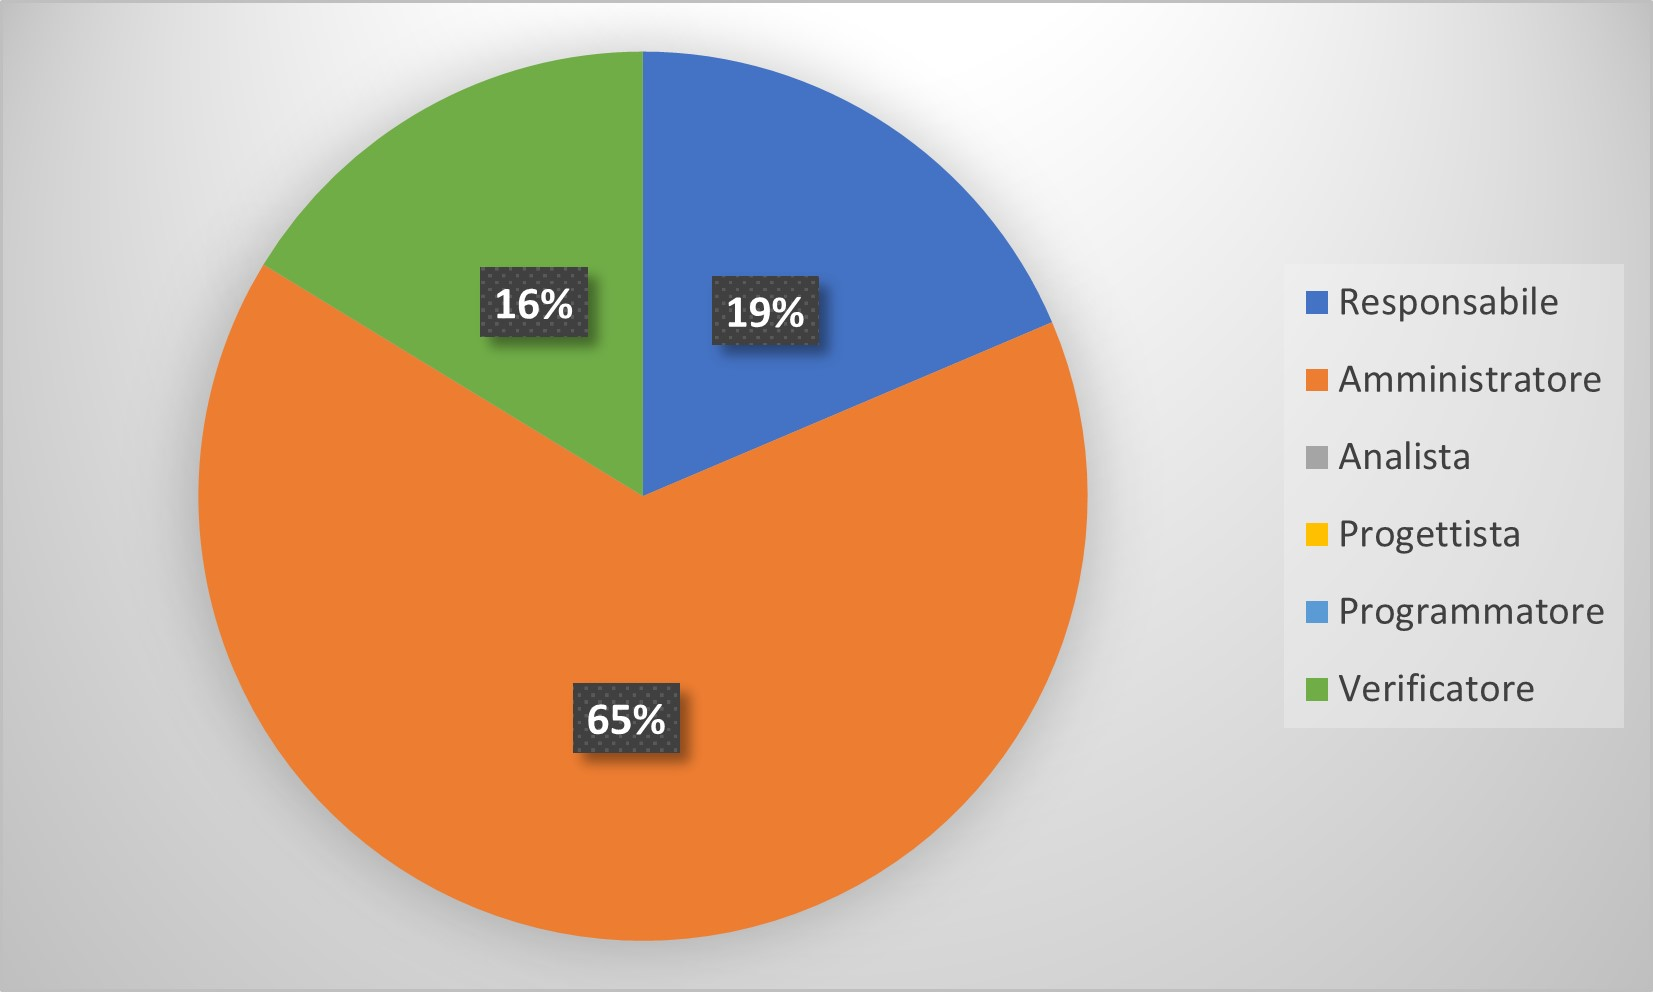
\includegraphics[width=1.0\textwidth]{Torta1.2.jpg}
    \caption{Grafico a torta della distribuzione dei costi}
\end{figure}

\newpage
\subsection{Secondo periodo}

In questa fase i ruoli da ricoprire per portare a termine gli obiettivi
pianificati sono:
\begin{itemize}
    \item \textit{Responsabile};
    \item \textit{Amministratore};
    \item \textit{Analista};
    \item \textit{Verificatore}.
\end{itemize}

\subsubsection{Preventivo orario}

\begin{table}[H]
    \centering
    \begin{tabular}{|l|c|c|c|c|c|c|c|}
    \hline
    \textbf{Membro} & \multicolumn{1}{l|}{\textbf{RE}} & \multicolumn{1}{l|}{\textbf{AM}} & \multicolumn{1}{l|}{\textbf{AN}} & \multicolumn{1}{l|}{\textbf{PT}} & \multicolumn{1}{l|}{\textbf{PR}} & \multicolumn{1}{l|}{\textbf{VE}} & \multicolumn{1}{l|}{\textbf{Totale ore persona}} \\ \hline
    \textit{Marco Mazzucato}  & - & 2   & 2  & - & - & 2  & 6   \\ \hline
    \textit{Marco Mamprin}    & - & 2   & 1  & - & - & 2  & 5   \\ \hline
    \textit{Marko Vukovic}    & - & 1.5 & 3  & - & - & 3  & 7.5 \\ \hline
    \textit{Mattia Zanellato} & - & -   & 3  & - & - & 3  & 6   \\ \hline
    \textit{Emanuele Pase}    & - & -   & 3  & - & - & 3  & 6   \\ \hline
    \textit{Riccardo Contin}  & 4 & -   & 3  & - & - & 1  & 8   \\ \hline
    \textit{Lorenzo Onelia}   & - & 2   & 2  & - & - & 3  & 7   \\ \hline
    \textbf{Totale ore ruolo} & 4 & 7.5 & 17 & - & - & 17 & 45.5\\ \hline
    \end{tabular}
    \caption{Distribuzione delle ore per la seconda milestone}
\end{table}

\begin{figure}[H]
    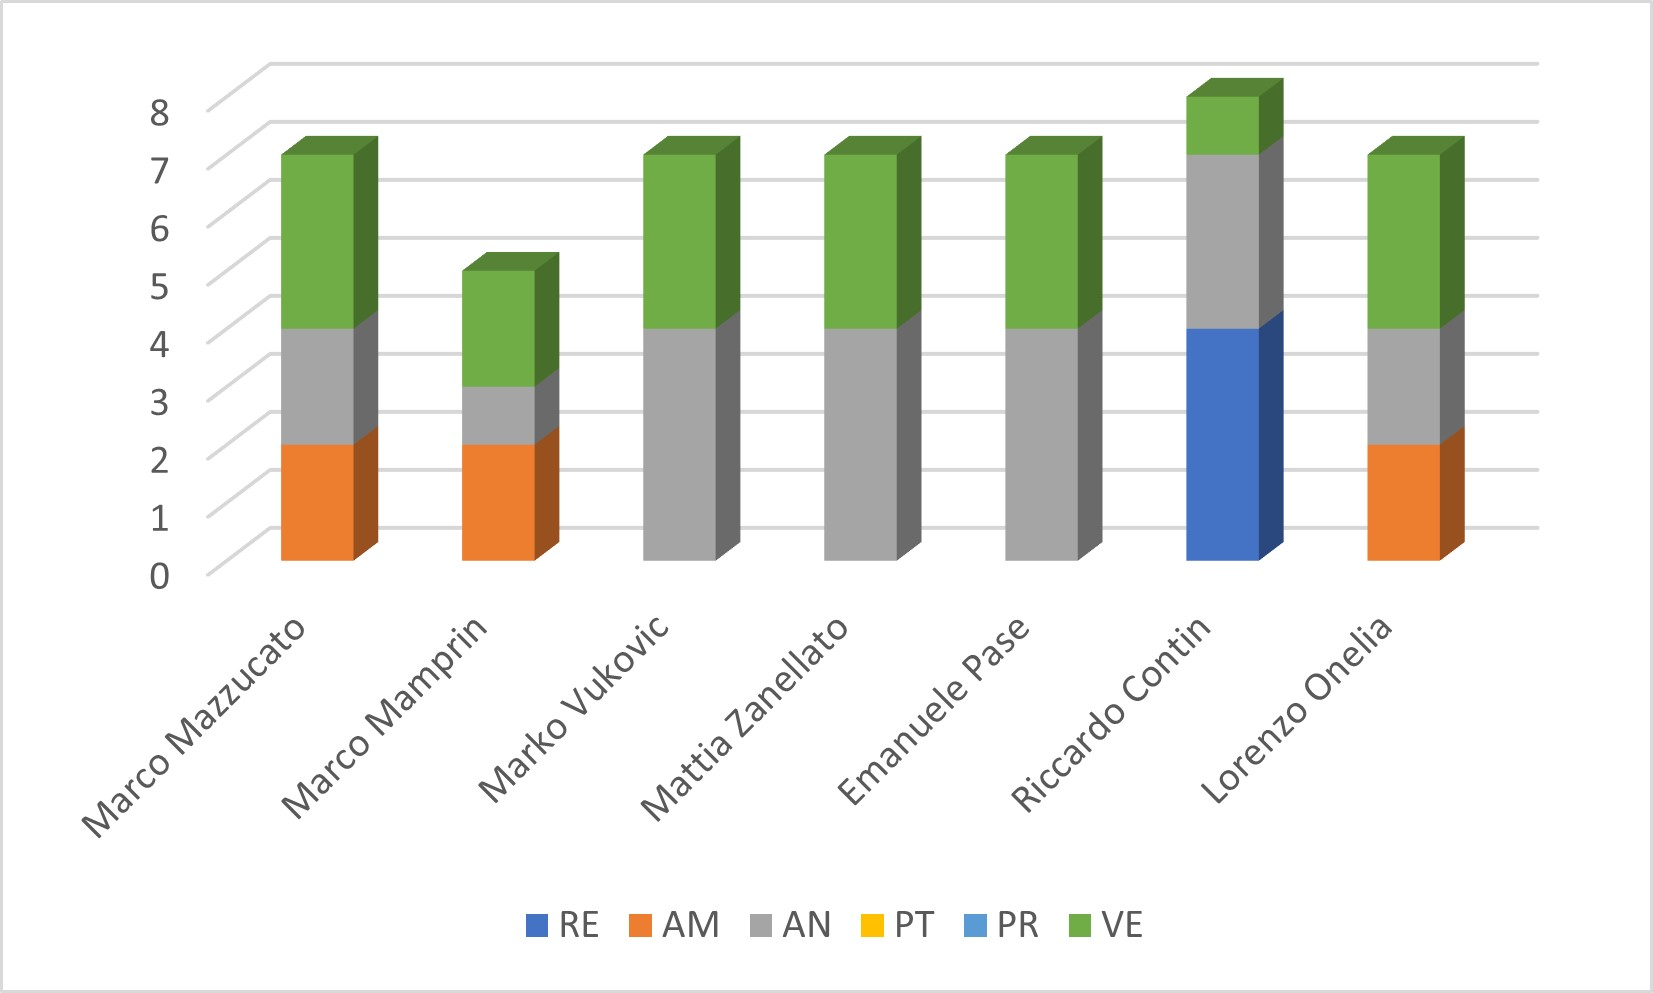
\includegraphics[width=1.0\textwidth]{Istogramma2.jpg}
    \caption{Istogramma della distribuzione delle ore}
\end{figure}

\begin{figure}[H]
    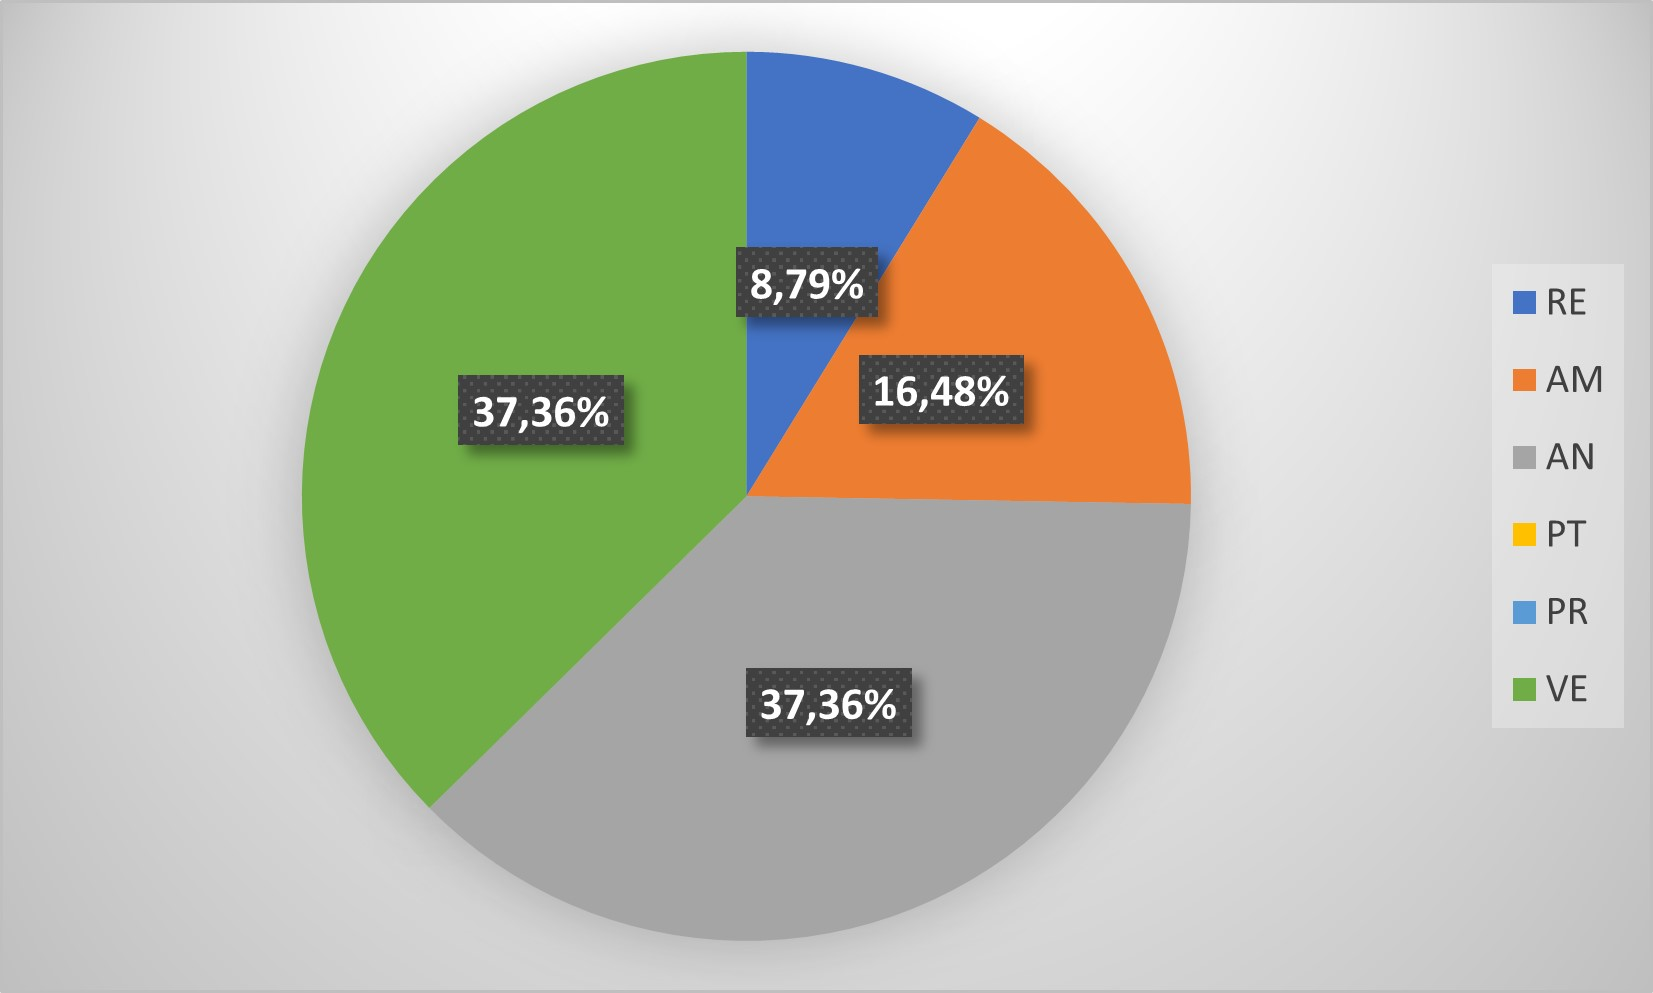
\includegraphics[width=1.0\textwidth]{Torta2.1.jpg}
    \caption{Grafico a torta della distribuzione delle ore}
\end{figure}

\newpage
\subsubsection{Preventivo economico}

\begin{table}[H]
    \centering
    \begin{tabular}{|l|c|c|}
    \hline
    \textbf{Ruolo} & \multicolumn{1}{l|}{\textbf{Ore}} & \multicolumn{1}{l|}{\textbf{Costo (€)}} \\ \hline
    \textit{Responsabile} & 4 & 120 \\ \hline
    \textit{Amministratore} & 7.5 & 150 \\ \hline
    \textit{Analista} & 17 & 425 \\ \hline
    \textit{Progettista} & - & - \\ \hline
    \textit{Programmatore} & - & - \\ \hline
    \textit{Verificatore} & 17 & 255 \\ \hline
    \textbf{Totale} & 45.5 & 950 \\ \hline
    \end{tabular}
    \caption{Prospetto dei costi per la seconda milestone}
\end{table}

\begin{figure}[H]
    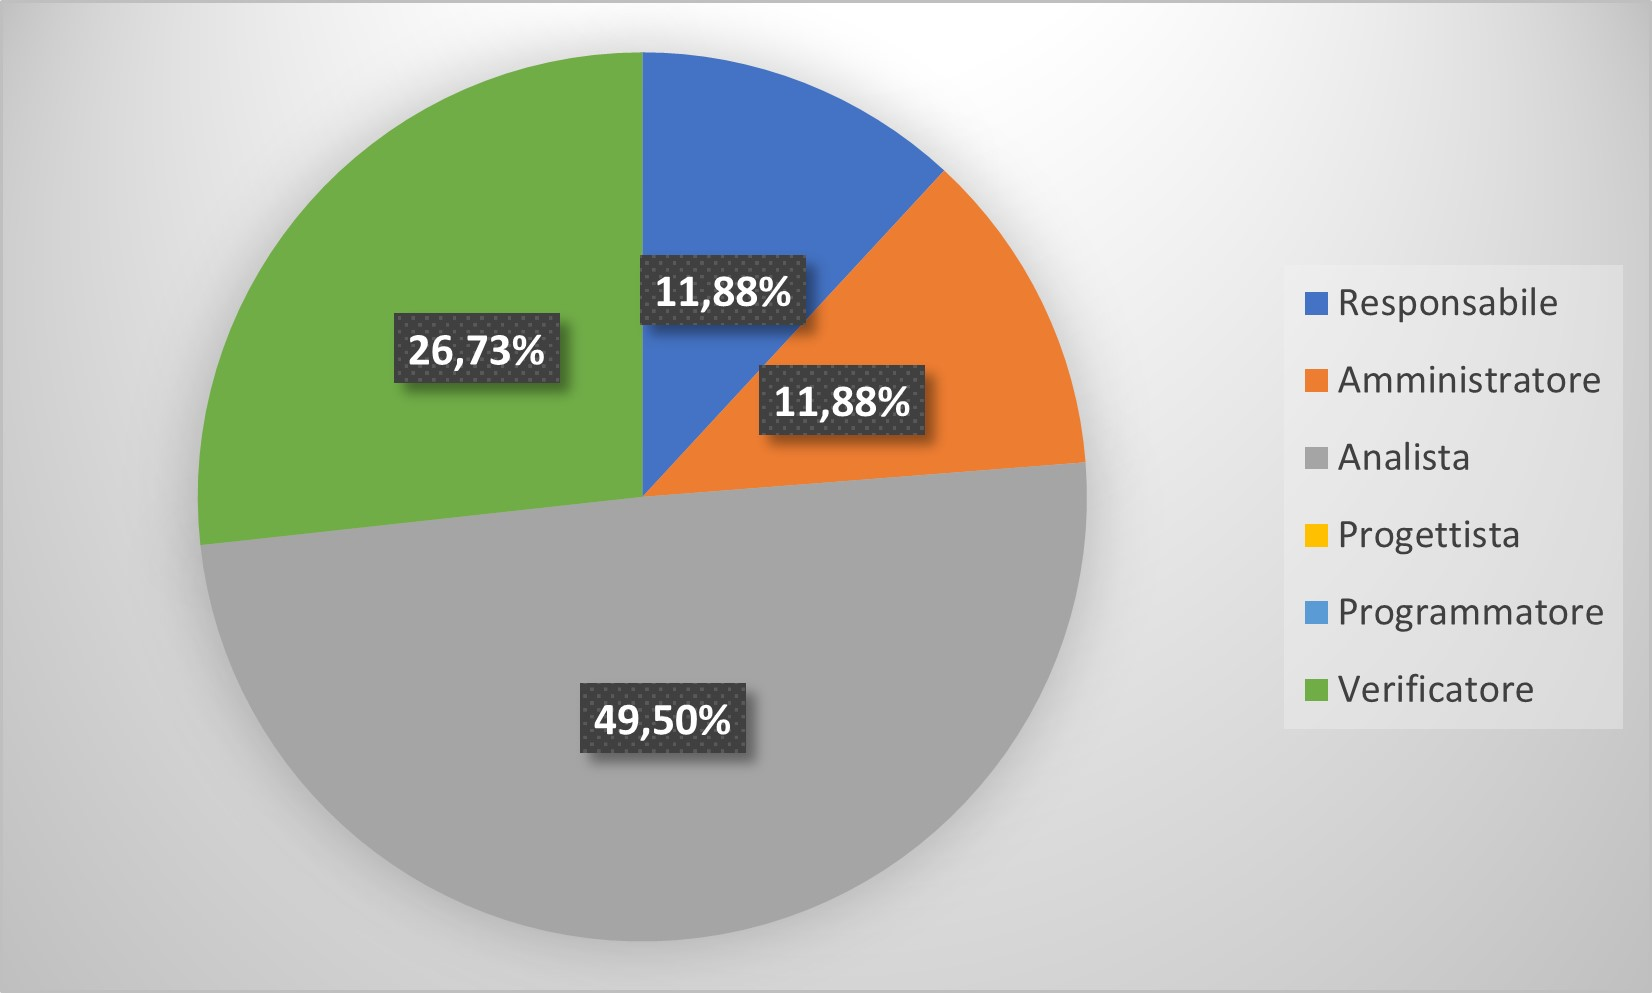
\includegraphics[width=1.0\textwidth]{Torta2.2.jpg}
    \caption{Grafico a torta della distribuzione dei costi}
\end{figure}



\newpage
\subsection{Terzo periodo}

In questa fase i ruoli da ricoprire per portare a termine gli obiettivi
pianificati sono:
\begin{itemize}
    \item \textit{Responsabile};
    \item \textit{Amministratore};
    \item \textit{Analista};
    \item \textit{Progettista};
    \item \textit{Verificatore}.
\end{itemize}

\subsubsection{Preventivo orario}

\begin{table}[H]
    \centering
    \begin{tabular}{|l|c|c|c|c|c|c|c|}
    \hline
    \textbf{Membro} & \multicolumn{1}{l|}{\textbf{RE}} & \multicolumn{1}{l|}{\textbf{AM}} & \multicolumn{1}{l|}{\textbf{AN}} & \multicolumn{1}{l|}{\textbf{PT}} & \multicolumn{1}{l|}{\textbf{PR}} & \multicolumn{1}{l|}{\textbf{VE}} & \multicolumn{1}{l|}{\textbf{Totale ore persona}} \\ \hline
    \textit{Marco Mazzucato}  & - & 1   & 1.5 & 2 & -  & 2    & 6.5  \\ \hline
    \textit{Marco Mamprin}    & - & 1   & 2   & 2 & -  & 2    & 7    \\ \hline
    \textit{Marko Vukovic}    & - & 1.5 & 2   & 2 & -  & 2    & 7.5  \\ \hline
    \textit{Mattia Zanellato} & - & 1   & 2   & 2 & -  & 2    & 7    \\ \hline
    \textit{Emanuele Pase}    & 4 & 1   & 0.5 & 2 & -  & 1    & 8.5  \\ \hline
    \textit{Riccardo Contin}  & - & 1   & 1.5 & 2 & -  & 2.5  & 7    \\ \hline
    \textit{Lorenzo Onelia}   & - & 1   & 1.5 & 2 & -  & 2    & 6.5  \\ \hline
    \textbf{Totale ore ruolo} & 4 & 7.5 & 11  & 14& - & 13.5 & 50   \\ \hline
    \end{tabular}
    \caption{Distribuzione delle ore per la terza milestone}
\end{table}

\begin{figure}[H]
    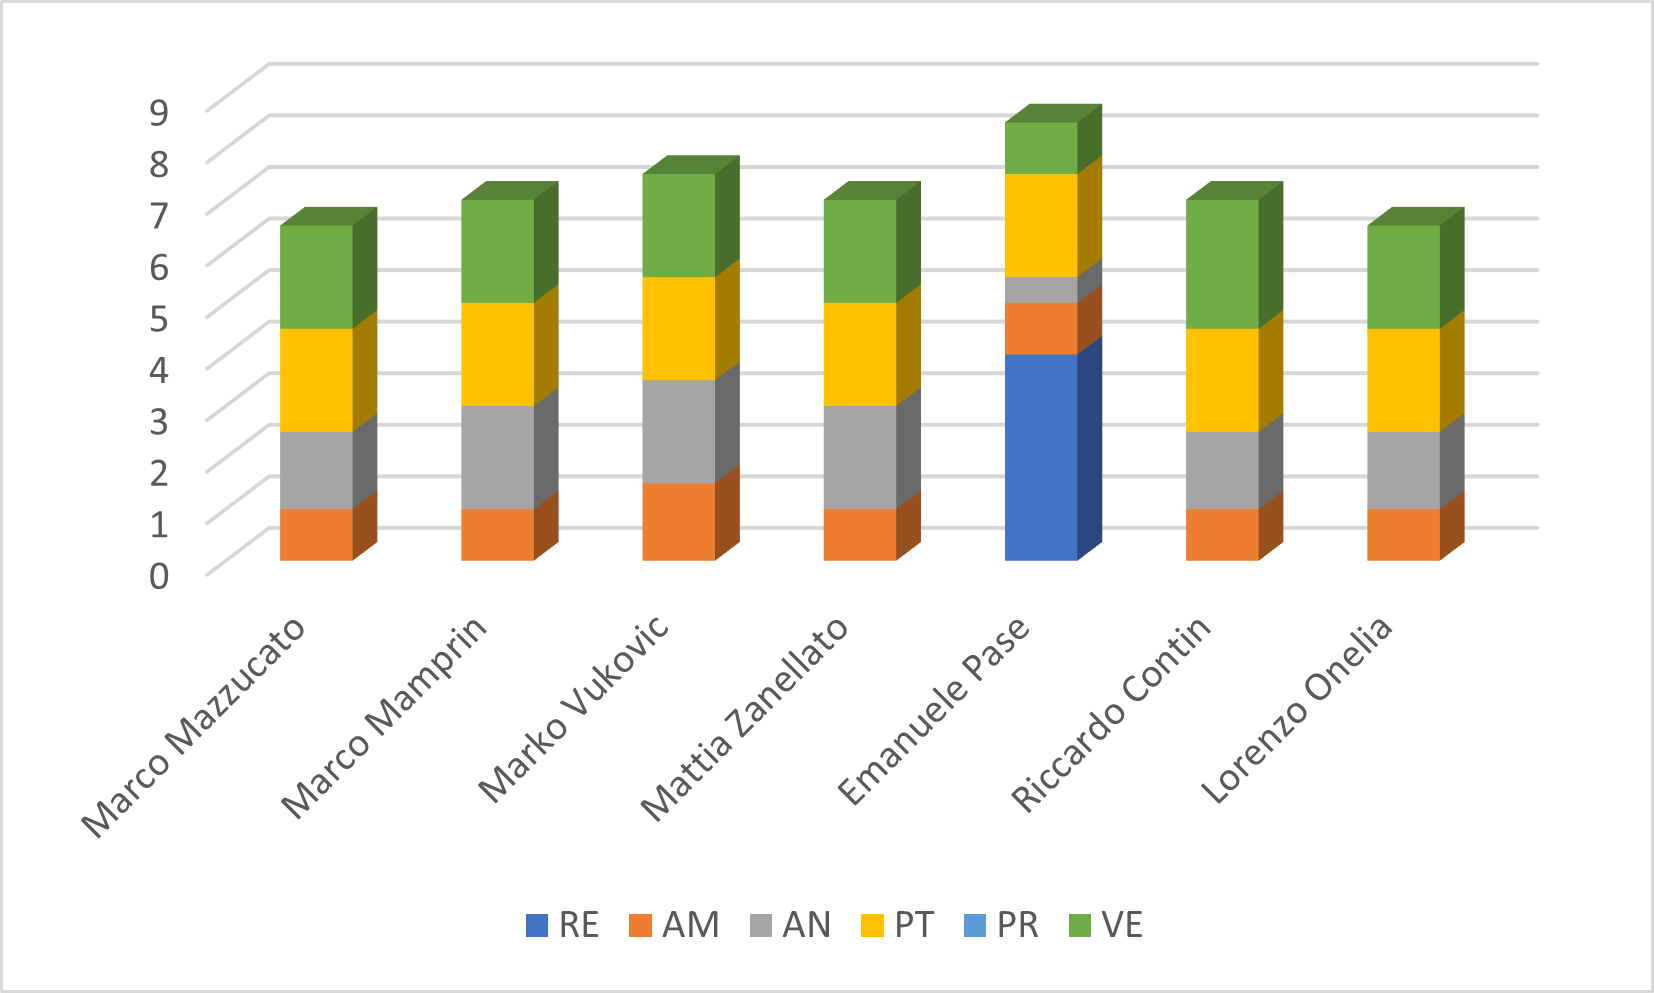
\includegraphics[width=1.0\textwidth]{Istogramma3.jpg}
    \caption{Istogramma della distribuzione delle ore}
\end{figure}

\begin{figure}[H]
    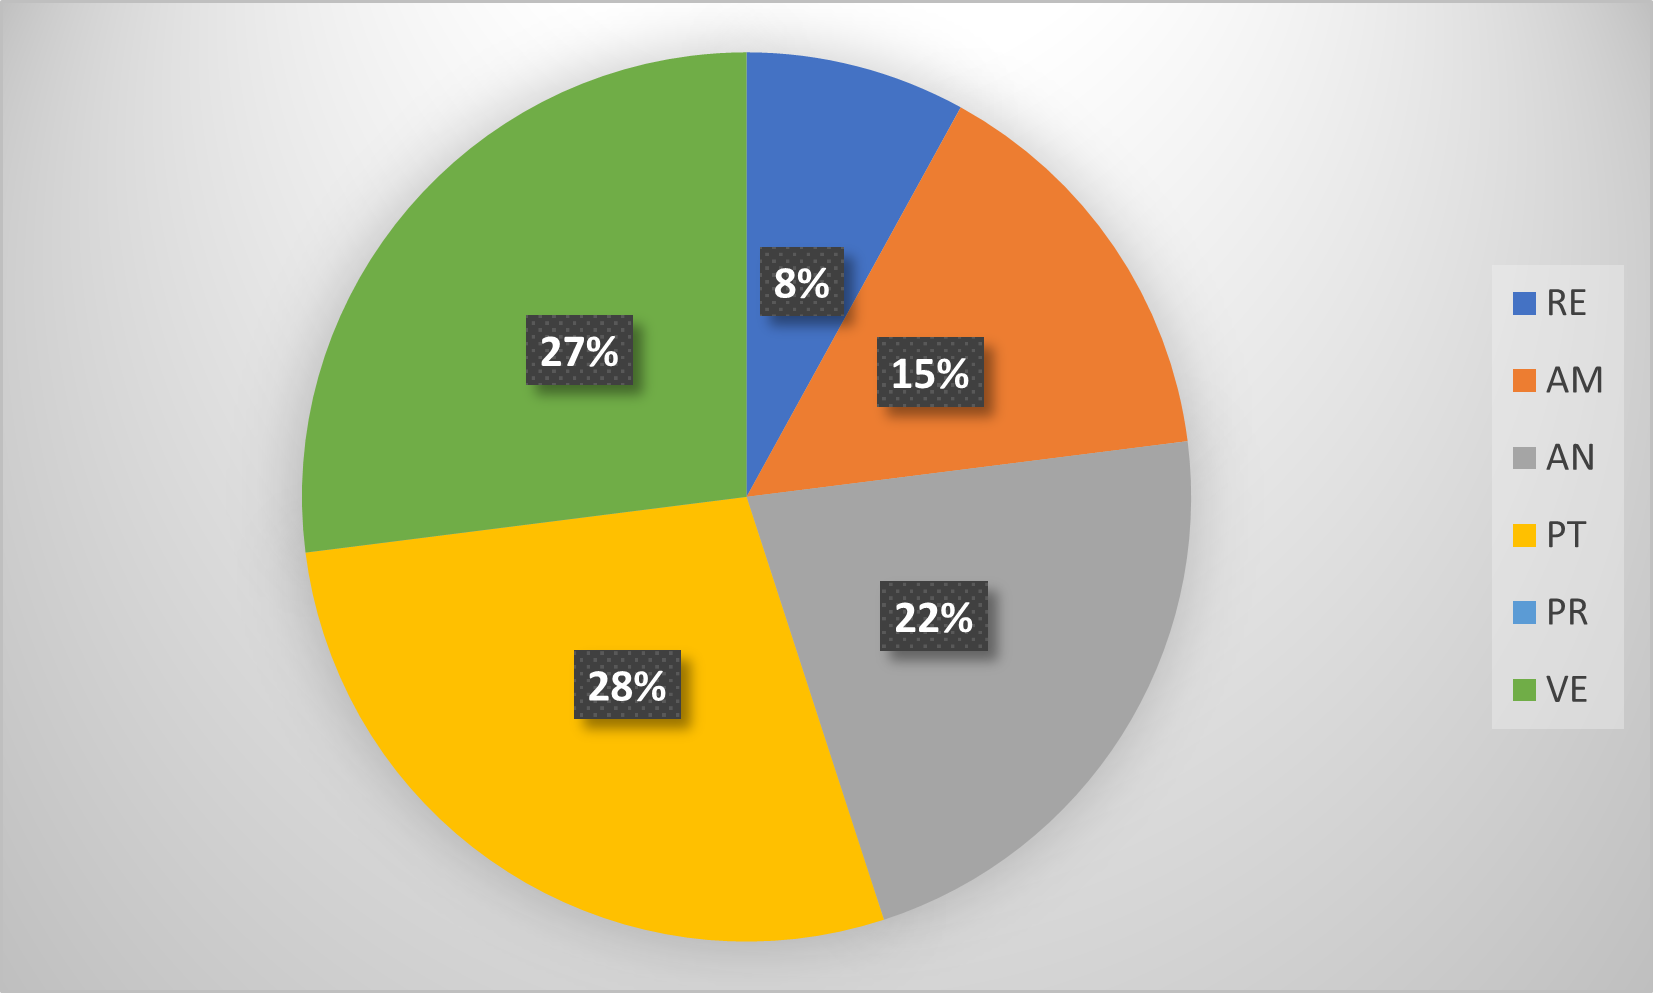
\includegraphics[width=1.0\textwidth]{Torta3.1.jpg}
    \caption{Grafico a torta della distribuzione delle ore}
\end{figure}

\newpage
\subsubsection{Preventivo economico}

\begin{table}[H]
    \centering
    \begin{tabular}{|l|c|c|}
    \hline
    \textbf{Ruolo} & \multicolumn{1}{l|}{\textbf{Ore}} & \multicolumn{1}{l|}{\textbf{Costo (€)}} \\ \hline
    \textit{Responsabile}   & 4    & 120   \\ \hline
    \textit{Amministratore} & 7.5  & 150   \\ \hline
    \textit{Analista}       & 11   & 275   \\ \hline
    \textit{Progettista}    & 14   & 350   \\ \hline
    \textit{Programmatore}  & -    & -     \\ \hline
    \textit{Verificatore}   & 13.5 & 202.5 \\ \hline
    \textbf{Totale}         & 50   & 1097,5\\ \hline
    \end{tabular}
    \caption{Prospetto dei costi per la terza milestone}
\end{table}

\begin{figure}[H]
    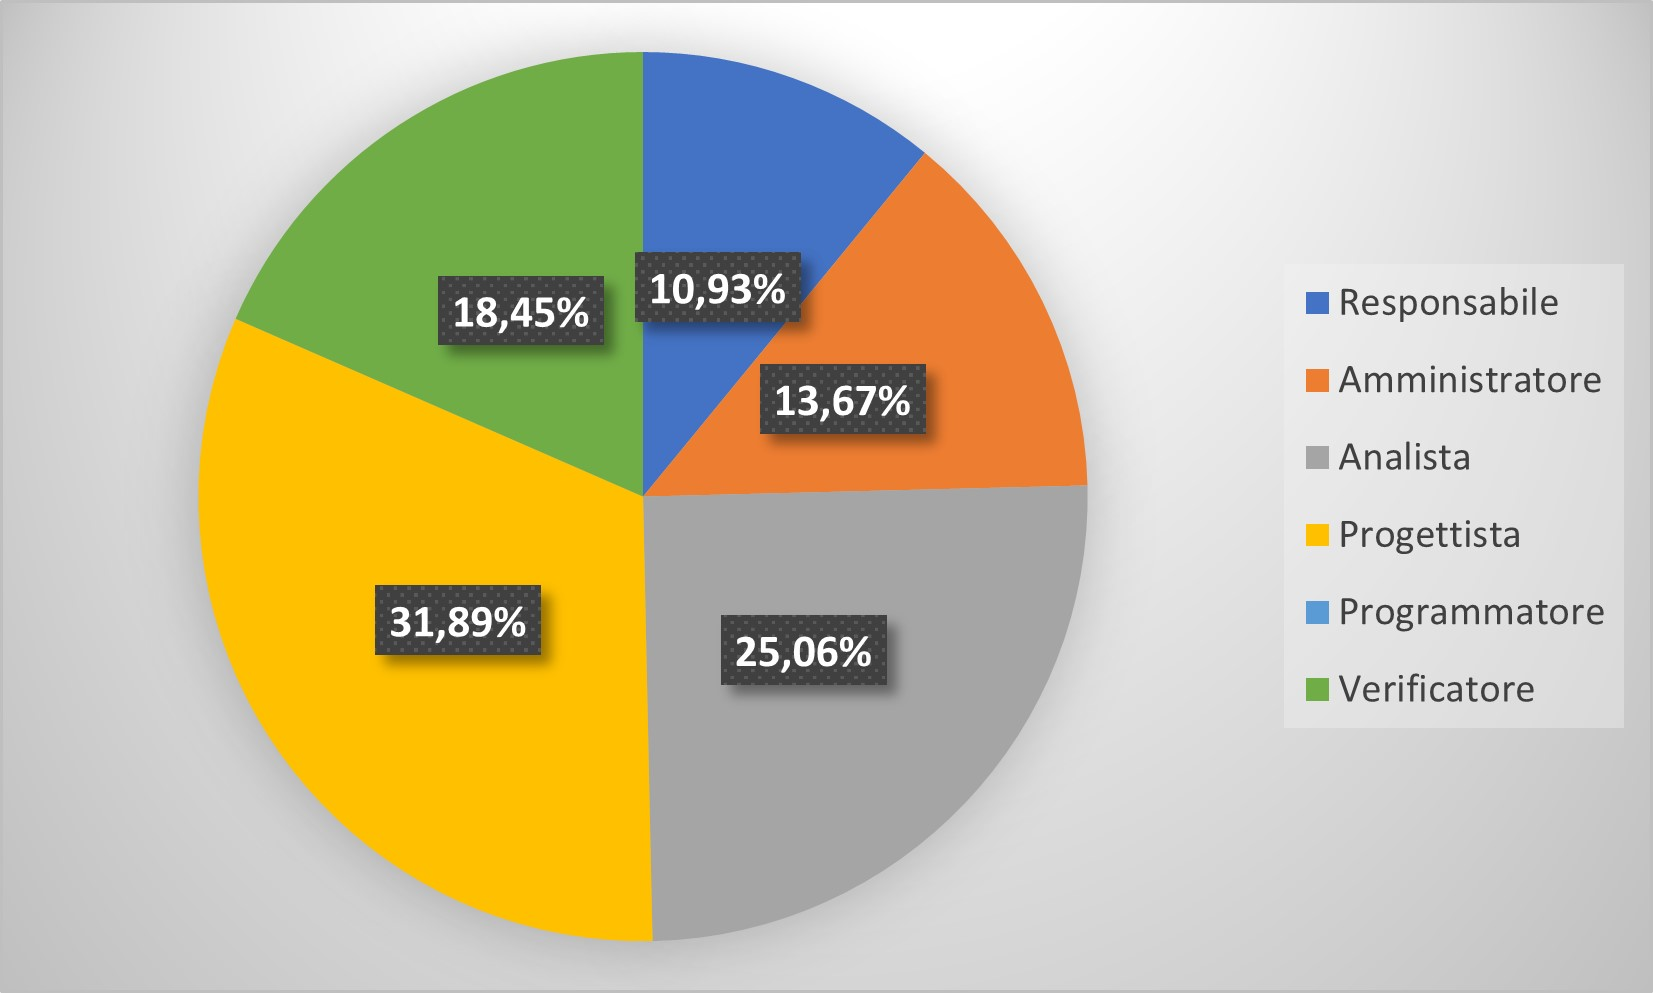
\includegraphics[width=1.0\textwidth]{Torta3.2.jpg}
    \caption{Grafico a torta della distribuzione dei costi}
\end{figure}



\newpage
\subsection{Quarto periodo}

In questa fase i ruoli da ricoprire per portare a termine gli obiettivi pianificati sono:
\begin{itemize}
    \item \textit{Responsabile};
    \item \textit{Amministratore};
    \item \textit{Analista};
    \item \textit{Progettista};
    \item \textit{Programmatore};
    \item \textit{Verificatore}.
\end{itemize}

\subsubsection{Preventivo orario}

\begin{table}[H]
    \centering
    \begin{tabular}{|l|c|c|c|c|c|c|c|}
    \hline
    \textbf{Membro} & \multicolumn{1}{l|}{\textbf{RE}} & \multicolumn{1}{l|}{\textbf{AM}} & \multicolumn{1}{l|}{\textbf{AN}} & \multicolumn{1}{l|}{\textbf{PT}} & \multicolumn{1}{l|}{\textbf{PR}} & \multicolumn{1}{l|}{\textbf{VE}} & \multicolumn{1}{l|}{\textbf{Totale ore persona}} \\ \hline
    \textit{Marco Mazzucato}  & - & -   & 2     & 4  & 4   & 2    & 12     \\ \hline
    \textit{Marco Mamprin}    & - & 1   & 2     & 4  & 5   & 3    & 15     \\ \hline
    \textit{Marko Vukovic}    & - & -   & 1     & 4  & 4   & 4    & 13     \\ \hline
    \textit{Mattia Zanellato} & 4 & 4   & 1.5   & 4  & -   & 4    & 17.5   \\ \hline
    \textit{Emanuele Pase}    & - & -   & -     & 3  & 4   & 3    & 10     \\ \hline
    \textit{Riccardo Contin}  & - & 3   & 1     & 3  & -   & 3.5  & 10.5   \\ \hline
    \textit{Lorenzo Onelia}   & - & 3   & 3     & 3  & -   & 3    & 12     \\ \hline
    \textbf{Totale ore ruolo} & 4 & 11  & 10.5  & 25 & 17  & 22.5 & 90     \\ \hline
    \end{tabular}
    \caption{Distribuzione delle ore per la quarta milestone}
\end{table}

\begin{figure}[H]
    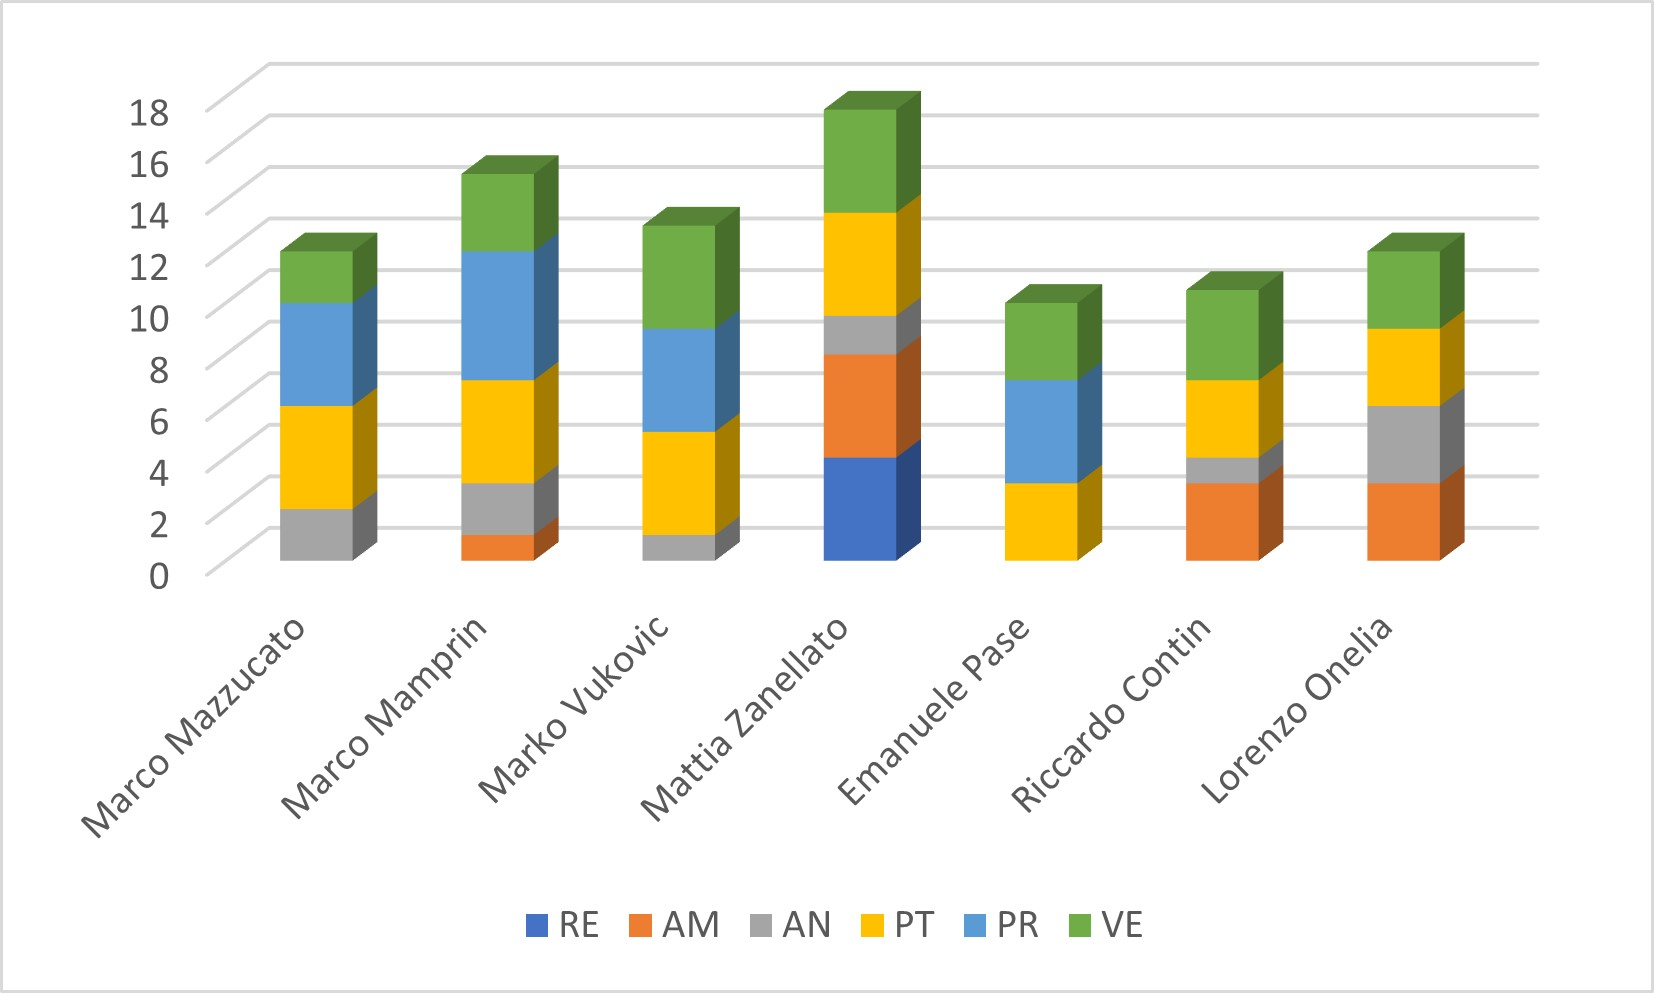
\includegraphics[width=1.0\textwidth]{Istogramma4.jpg}
    \caption{Istogramma della distribuzione delle ore}
\end{figure}

\begin{figure}[H]
    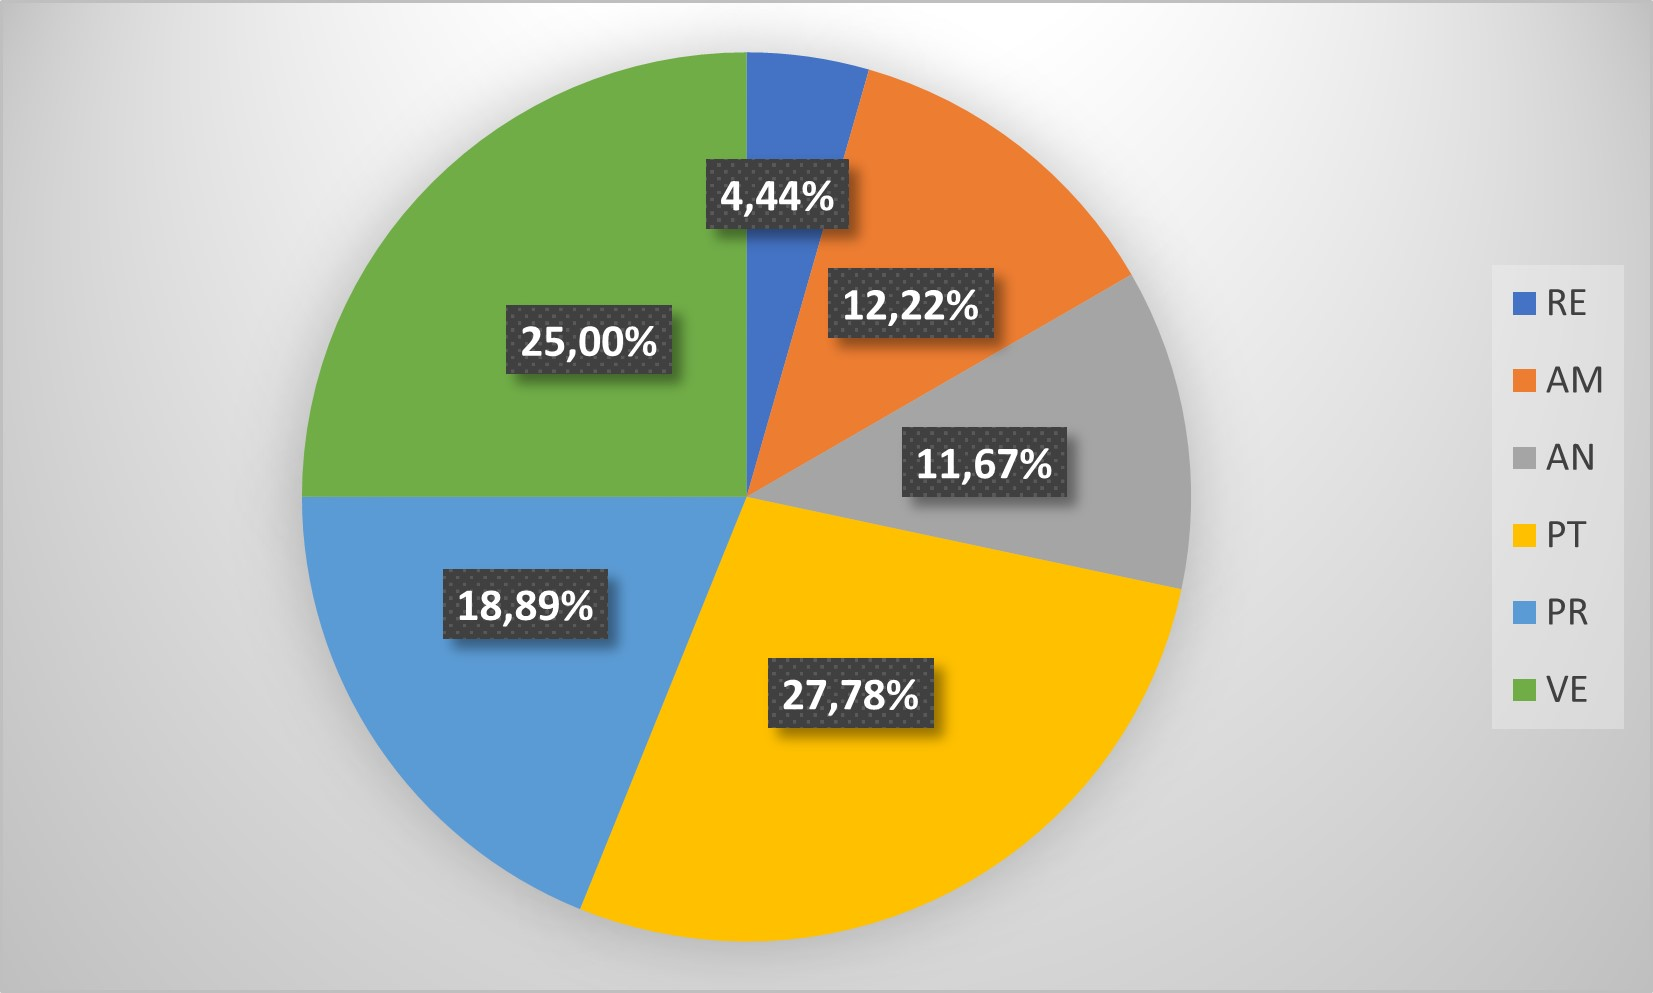
\includegraphics[width=1.0\textwidth]{Torta4.1.jpg}
    \caption{Grafico a torta della distribuzione delle ore}
\end{figure}

\newpage
\subsubsection{Preventivo economico}

\begin{table}[H]
    \centering
    \begin{tabular}{|l|c|c|}
    \hline
    \textbf{Ruolo} & \multicolumn{1}{l|}{\textbf{Ore}} & \multicolumn{1}{l|}{\textbf{Costo (€)}} \\ \hline
    \textit{Responsabile}   & 4    & 120     \\ \hline
    \textit{Amministratore} & 11   & 220     \\ \hline
    \textit{Analista}       & 10.5 & 262.5   \\ \hline
    \textit{Progettista}    & 25   & 625     \\ \hline
    \textit{Programmatore}  & 17   & 255     \\ \hline
    \textit{Verificatore}   & 22.5 & 337.5   \\ \hline
    \textbf{Totale}         & 90   & 1820    \\ \hline
    \end{tabular}
    \caption{Prospetto dei costi per la quarta milestone}
\end{table}

\begin{figure}[H]
    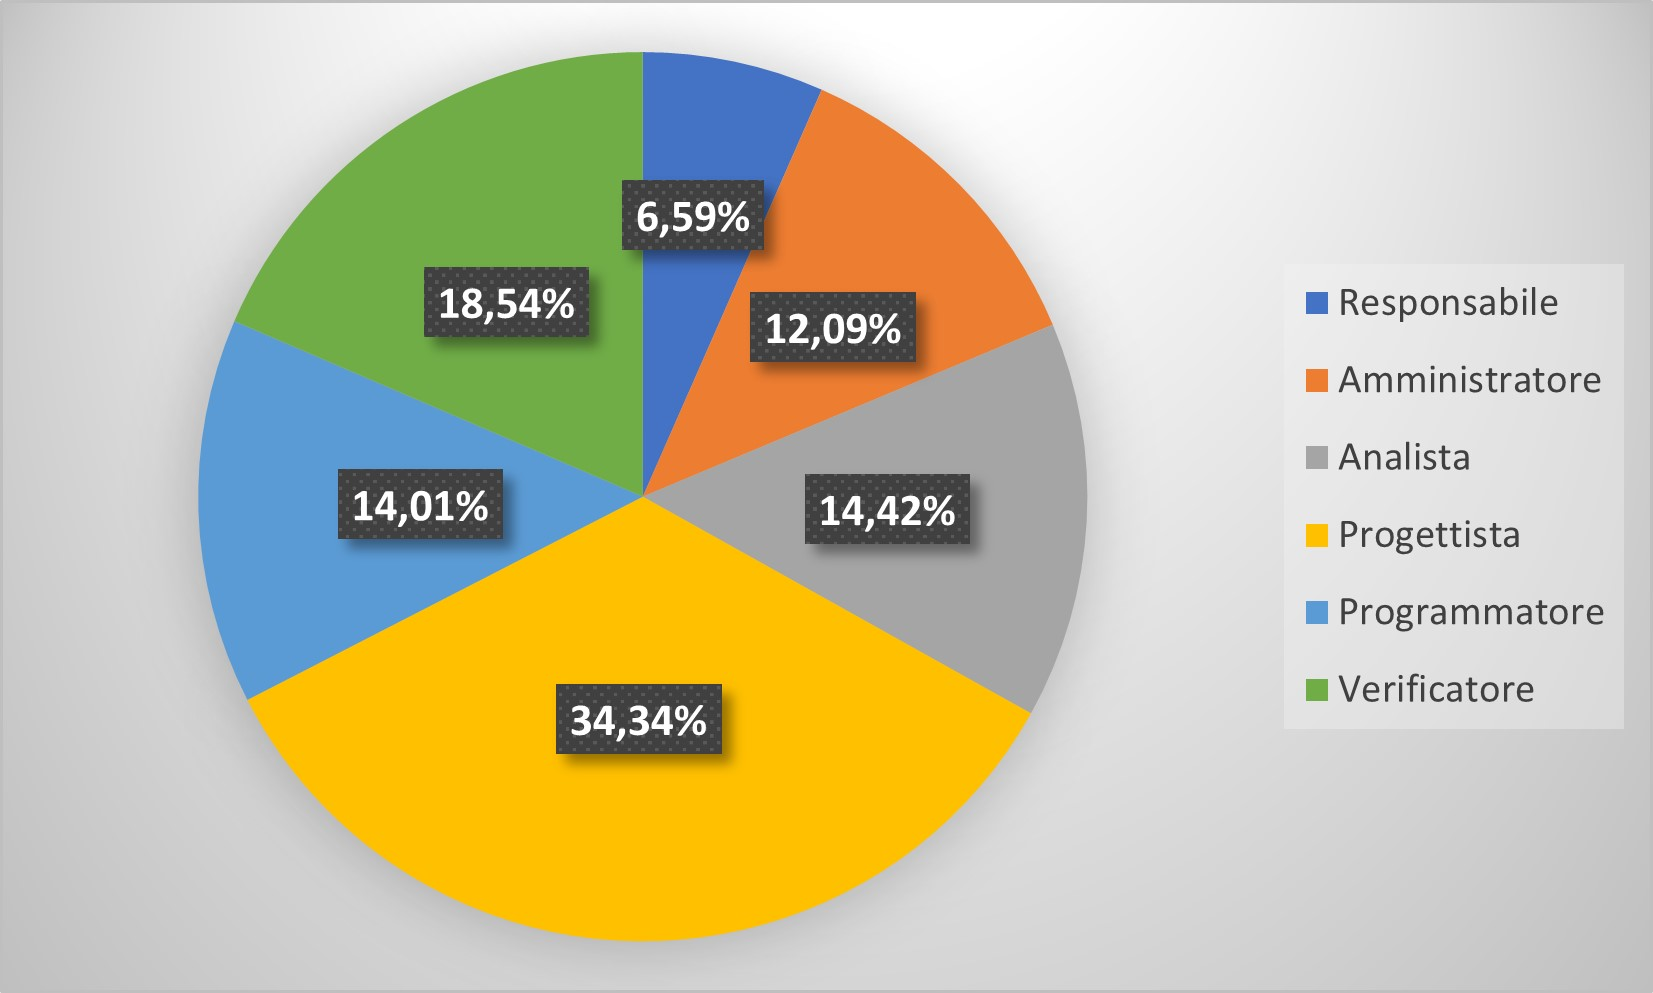
\includegraphics[width=1.0\textwidth]{Torta4.2.jpg}
    \caption{Grafico a torta della distribuzione dei costi}
\end{figure}


\section{Verso la PB}

\section{Verso la CA}
